\newpage
\hypertarget{allCards vis}{}
\subsection{AllOtherPartitionsRule}
\genHeader

\begin{itemize}

\item[$\blacktriangleright$] Create a new rule \texttt{AllOtherPartitionsRule}, and complete it according to Fig.~\ref{fig:ea_AllOtherPartitionsRuleComplete}.


\begin{figure}[htbp]
\begin{center}
  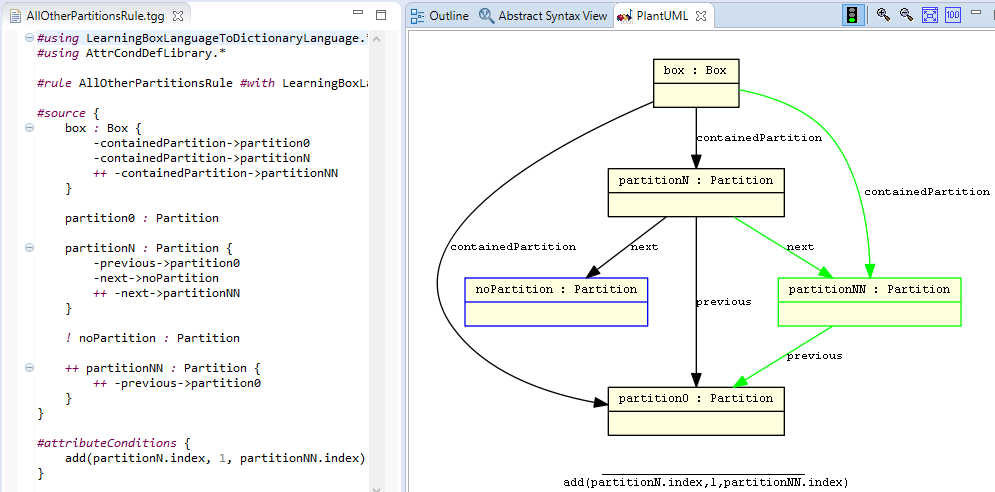
\includegraphics[width=\textwidth]{ea_AllOtherPartitionsRule}
  \caption{The completed \texttt{AllOtherPartitionsRule}}
  \label{fig:ea_AllOtherPartitionsRuleComplete}
\end{center}
\end{figure}

\item[$\blacktriangleright$] As you can see, this rule doesn't assume to know the final \texttt{partition} in the transformation. 
It matches the \texttt{n}th partition as the partition without any next partition, then connects a new \texttt{n+1}th partition to \texttt{n} and \texttt{partition0} (clear as every partitions previous is \texttt{partition0}).
Note that TGG transformations assume that the models are valid, i.e., have the expected structure (in our case meaning that the learning box is correctly ``wired'').\footnote{This should actually be formalised with a set of metamodel constraints that must be checked before a transformation is run, but we've omitted this here to simplify things.}  
Remember that ``blue'' means ``negative''.

\item[$\blacktriangleright$] Generate code for your improved TGG and re-run the transformation. 
It should work now without any error message.
Inspect the protocol to understand what happened.

\item[$\blacktriangleright$] Go ahead and add as many \texttt{partition}s and \texttt{card}s as you like to your model instance.
Your TGG is now also able to handle a \texttt{box} with any number of \texttt{partition}s beautifully.
For five partitions all with cards, the protocol gets quite interesting and is no longer a flat tree.
Try it out! 

\end{itemize}



%%% Local Variables: 
%%% mode: latex
%%% TeX-master: "../src/TGG_mainFile"
%%% End: 
